\section{Clase 1}

\title[Circuitos Discretos]{Circuitos Discretos}
\subtitle{Clase 1: Repaso BJT}
\institute[]{Instituto Tecnológico de Costa Rica\\Escuela de Ingeniería Electrónica\\Circuitos Discretos}
\date{\theSemester}
\titlegraphic{
\includegraphics[height=8mm]{logoTEC.png}}

\begin{frame}[t]
\titlepage
\end{frame}

\begin{frame}[t]
\frametitle{El transistor BJT}

\begin{multicols}{2}
    El transistor de unión bipolar está formado por tres regiones de silicio:

    \begin{itemize}
        \item Base
        \item Colector
        \item Emisor
    \end{itemize}
    
    \begin{figure}[H]
        \centering
        \begin{circuitikz}
            \draw (0,0) node[npn]{};
            \draw (2,0) node[pnp]{};
        \end{circuitikz}
        \caption{Símbolos del transistor BJT.}
        \label{bjtsymbols}
    \end{figure}

    \begin{figure}[H]
        \centering
        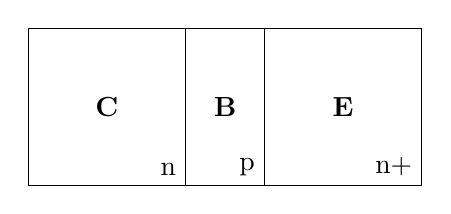
\begin{tikzpicture}
            \draw (0,0) rectangle (5,2);
            \draw (2,0) -- (2,2);
            \draw (3,0) -- (3,2);
            \draw (1,1) node[]{\textbf{C}};
            \draw (2.5,1) node[]{\textbf{B}};
            \draw (4,1) node[]{\textbf{E}};
            \draw (2,0) node[anchor=south east]{n};
            \draw (3,0) node[anchor=south east]{p};
            \draw (5,0) node[anchor=south east]{n+};
        \end{tikzpicture}
        \caption{Estructura del transistor BJT NPN.}
        \label{bjtstructure}
    \end{figure}

    \begin{center}
        \textbf{Las terminales del emisor y el colector NO son intercambiables.}
    \end{center}
\end{multicols}

En un transistor BJT típico:

\begin{itemize}
    \item El emisor tiene un dopado más alto que el colector.
    \item La base es mucho más delgada que las otras dos regiones.    
\end{itemize}

\end{frame}


\begin{frame}[t]
    \frametitle{El transistor BJT: Funcionamiento en Activa Directa}
    
    \begin{multicols}{2}
        \begin{circuitikz}[american,scale=0.8]
            \draw (0,0) rectangle (2,5);
            \draw (0,2) -- (2,2);
            \draw (0,3) -- (2,3);
            \draw (-1.5,2.5) to[V,l=$V_{BE}$] (-1.5,0);
            \draw (-1.5,2.5) -- (0,2.5);
            \draw (-1.5,0) node[ground]{};
            \draw (3.5,4) to[V,l=$V_{CE}$] (3.5,0);
            \draw (3.5,4) -- (2,4);
            \draw (3.5,0) node[ground]{};
            \draw (1,1) node[]{\textbf{E}};
            \draw (1,2.5) node[]{\textbf{B}};
            \draw (1,4) node[]{\textbf{C}};
            \draw (2,0) node[anchor=south east]{n+};
            \draw (2,2) node[anchor=south east]{p};
            \draw (2,3) node[anchor=south east]{n};
        \end{circuitikz}

        En la región \textbf{activa directa}:

        \begin{itemize}
            \item El diodo B-E está polarizado en directa, con una tensión mayor a 0.7 V
            \item El diodo B-C está polarizado en reversa, con una tensión B-C negativa.
        \end{itemize}

        La corriente de base (corriente convencional) hace que los electrones que vienen del emisor lleguen a la base, y sean recolectados por el colector.
    \end{multicols}

    Si la tensión $V_{CE}$ cae por debajo de la tensión $V_{BE}$, el transistor se encuentra en \textbf{saturación}.

    Sin embargo, puede considerarse que existe \textbf{saturación débil} si se cumple que $V_{CE} > V_{BE} - 200 mV$ (el diodo B-C aun está apagado en esta región).
\end{frame}

\begin{frame}[t]
    \frametitle{El transistor BJT: Curva de Transferencia}

    \begin{multicols}{2}
        La \textbf{curva de transferencia} se mide al dejar $V_{CE}$ constante y modificar $V_{BE}$.

        \vspace{5mm}
        \begin{figure}[H]
            \begin{circuitikz}
                \draw (0,0) node[npn](npn1){};
                \draw (-2,0) to[battery1,l=$V_{BE}$] (-2,-1);
                \draw (-2,-1) node[ground]{};
                \draw (-2,0) -- (npn1.base);
                \draw (0,-1) node[ground]{};
                \draw (0,-1) -- (npn1.emitter);
                \draw (2,1) to[V,l=$V_{CE}$] (2,-1);
                \draw (2,1) -- (0,1);
                \draw (0,1) -- (npn1.collector);
                \draw (2,-1) node[ground]{};
                \draw [->] (-2.25,-0.75) -- (-1.75,-0.25);
            \end{circuitikz}
            %\caption{Circuito de medición de la curva de transferencia.}
            %\label{tfcircuit}
        \end{figure}
        
        \vspace{5mm}
        Esta curva está descrita por la ecuación de Shockley:

        \[ I_C = I_S (e^{V_{BE}/V_t}-1)(1+V_{CE}/V_A) \]

        \newpage
        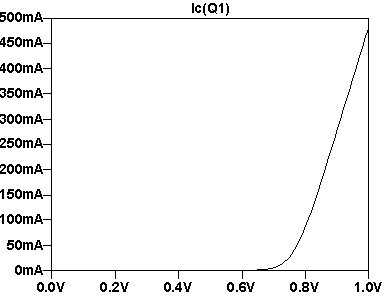
\includegraphics[width=5.5cm]{BJT_transfer.pdf}

    \end{multicols}
\end{frame}

\begin{frame}[t]
    \frametitle{El transistor BJT: Curva de Salida}

    \begin{multicols}{2}
        La \textbf{curva de salida} se mide al mantener $V_{BE}$ constante y variar $V_{CE}$.

        \vspace{5mm}
        \begin{figure}[H]
            \begin{circuitikz}
                \draw (0,0) node[npn](npn1){};
                \draw (-2,0) to[V,l=$V_{BE}$] (-2,-1);
                \draw (-2,-1) node[ground]{};
                \draw (-2,0) -- (npn1.base);
                \draw (0,-1) node[ground]{};
                \draw (0,-1) -- (npn1.emitter);
                \draw (2,1) to[battery1,l=$V_{CE}$] (2,-1);
                \draw (2,1) -- (0,1);
                \draw (0,1) -- (npn1.collector);
                \draw (2,-1) node[ground]{};
                \draw [->] (1.75,-0.25) -- (2.25,0.25);
            \end{circuitikz}
            %\caption{Circuito de medición de la curva de salida.}
            %\label{tfcircuit2}
        \end{figure}

        \newpage
        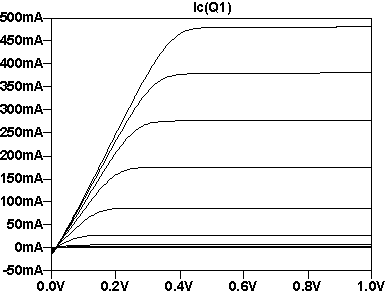
\includegraphics[width=5.5cm]{BJT_output.pdf}

    \end{multicols}

    En estas curvas se observa la diferencia entre la región de saturación y la región activa directa.

    \begin{itemize}
        \item Activa directa: funcionamiento como fuente de corriente
        \item Saturación: funcionamiento como resistencia
    \end{itemize}
\end{frame}


\begin{frame}[t]
    \frametitle{El transistor BJT: Efecto Early}

    El efecto Early se observa en la curva de salida.

    \begin{itemize}
        \item La tensión Early ($V_A$) se define como el punto donde todas las curvas interceptan el eje horizontal.
    \end{itemize}

    \begin{figure}
        \centering
        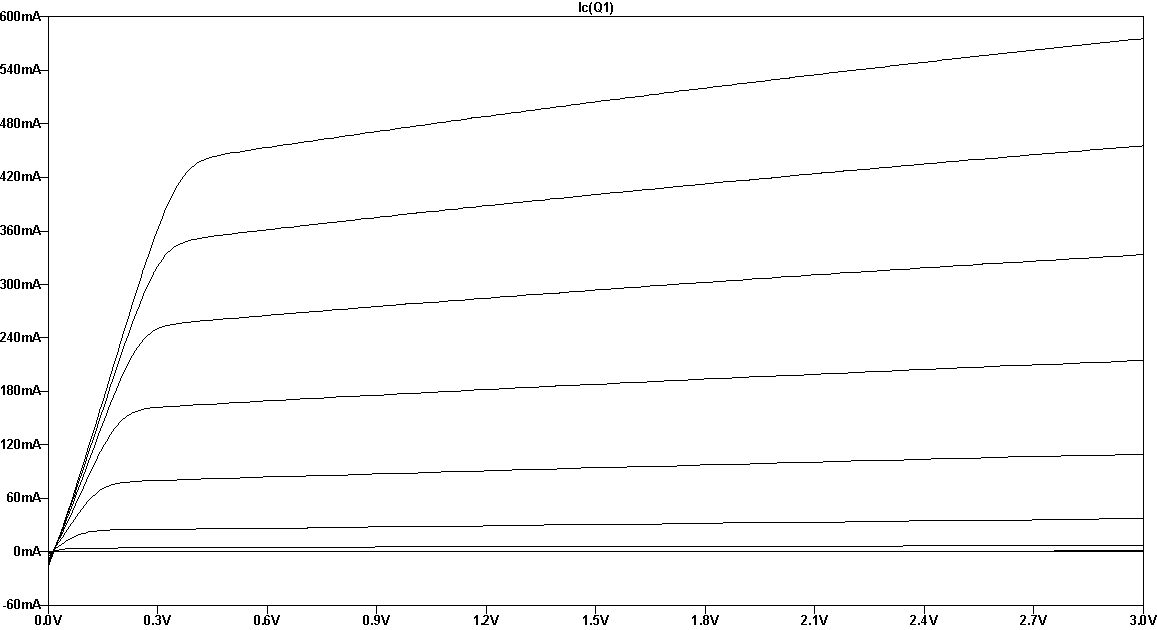
\includegraphics[width=0.6\textwidth]{BJT_early.pdf}
    \end{figure}


\end{frame}

\begin{frame}[t]
    \frametitle{El transistor BJT: Modelo de Gran Se\~{n}al}

    La corriente de colector se calcula por medio de la ecuación de Shockley:

    \[ I_C = I_S (e^{V_{BE}/V_t} - 1)(1 + V_{CE}/V_A) \]

    Se define la ganancia de corriente de emisor común:

    \[ I_C = \beta I_B \]

    Y la ganancia de corriente de base común:

    \[ I_E = \alpha I_C \]

    De manera que se cumple:

    \[ I_E = I_B + I_C \]

    \[ I_E = (\beta + 1) I_B \]

    \[ \alpha = \dfrac{\beta}{\beta+1} \]
\end{frame}


\begin{frame}[t]
    \frametitle{El transistor BJT: Polarización por Resistencia de Base}

    \begin{multicols}{2}
        \begin{figure}[H]
            \centering
            \begin{tikzpicture}
                \draw (0,2) node[npn](npn1){};
                \draw (-2,4) to[R,l=$R_B$] (-2,2){};
                \draw (-2,2) to[short] (npn1.base){};
                \draw (0,4) to[R, l=$R_C$] (npn1.collector){};
                \draw (0,1) node[ground]{};
                \draw (0,1) to[short] (npn1.emitter){};
                \draw (-2,5) to[short] (-2,4){};
                \draw (0,5) to[short] (0,4){};
                \draw (-2.5,5) to[short] (0.5,5);
                \draw (-1,5) node[anchor=south]{$V_{CC}$};
            \end{tikzpicture}
        \end{figure}


        La malla por la base:

        \[ V_{CC} = I_B R_B + V_{BE} \]

        \[ I_B = \dfrac{V_{CC}-V_{BE}}{R_B} \]

        \[ I_C = \beta \left( \dfrac{V_{CC}-V_{BE}}{R_B} \right) \]

        La ecuación de Shockley:

        \[ I_C = I_S (e^{V_{BE}/V_t} - 1) \]

        Este es un sistema de ecuaciones de dos variables.

        \begin{itemize}
            \item Solución por método iterativo
            \item Solución por aproximación numérica
        \end{itemize}
    \end{multicols}
\end{frame}

\begin{frame}[t]
    \frametitle{El transistor BJT: Soluciones del Sistema de Ecuaciones}

    \begin{multicols}{2}
        \textbf{Por método iterativo}

        \begin{enumerate}
            \item Suponer un valor inicial para $V_{BE}$
            \item Calcular $I_C$ con la ecuación de malla
            \item Recalcular $V_{BE}$ con la ecuación de Shockley
            \item Repetir 2. y 3. hasta minimizar el error
        \end{enumerate}
        
        El error en $I_C$ para cada iteración se calcula como:

        \[ \epsilon = \dfrac{I_{C} - I_{C-1}}{I_C} \times 100\% \]

        \newpage
        \textbf{Por aproximación numérica}

        Despejando $V_{BE}$ de la ecuación de Shockley:

        \[ V_{BE} = V_t ln {\dfrac{I_C}{I_S}} \]

        Sustituyendo en la ecuación de malla:

        \[ I_C = \beta \left( \dfrac{V_{CC}-V_t ln (I_C/I_S)}{R_B} \right) \]

        En esta ecuación no es posible despejar $I_C$, por lo tanto, se aproxima numéricamente en la calculadora.

    \end{multicols}
\end{frame}


\begin{frame}[t]
    \frametitle{El transistor BJT: Polarización por Divisor de Tensión}

    \begin{multicols}{2}
        \begin{figure}[H]
            \centering
            \begin{tikzpicture}
                \draw (0,2) node[npn](npn1){}
                (-2,4) to[R,l=$R_1$] (-2,2){}
                (-2,2) to[R,l=$R_2$] (-2,0){}
                (-2,0) node[ground]{}
                (-2,2) to[short] (npn1.base){}
                (0,4) to[R, l=$R_C$] (npn1.collector){}
                (0,0) node[ground]{}
                (0,0) to[short] (npn1.emitter){}
                (-2,5) to[short] (-2,4){}
                (0,5) to[short] (0,4){}
                (-2.5,5) to[short] (0.5,5)
                (-1,5) node[anchor=south]{$V_{CC}$}
                ;
            \end{tikzpicture}
        \end{figure}

        \newpage
        \textbf{Si la corriente de base es despreciable}

        \[ V_{BE} = \dfrac{V_{CC} \times R_2}{R_1 + R_2} \]

        \[ I_C = I_S (e^{V_{BE}/V_t}-1) \]
        
        \[ I_C = I_S (e^{\dfrac{1}{V_t} \cdot \dfrac{V_{CC} \times R_2}{R_1 + R_2}}-1) \]

        \begin{itemize}
            \item En esta configuración la corriente $I_C$ es independiente de $\beta$.
            \item Esto la hace muy estable ante variaciones de temperatura.
        \end{itemize}
        
    \end{multicols}

\end{frame} 


\begin{frame}[t]
    \frametitle{El transistor BJT: Polarización por Divisor de Tensión}

    \begin{multicols}{2}
        \begin{figure}[H]
            \centering
            \begin{tikzpicture}
                \draw (0,2) node[npn](npn1){}
                (-2,4) to[R,l=$R_1$] (-2,2){}
                (-2,2) to[R,l=$R_2$] (-2,0){}
                (-2,0) node[ground]{}
                (-2,2) to[short] (npn1.base){}
                (0,4) to[R, l=$R_C$] (npn1.collector){}
                (0,0) node[ground]{}
                (0,0) to[short] (npn1.emitter){}
                (-2,5) to[short] (-2,4){}
                (0,5) to[short] (0,4){}
                (-2.5,5) to[short] (0.5,5)
                (-1,5) node[anchor=south]{$V_{CC}$}
                ;
            \end{tikzpicture}
        \end{figure}

        \newpage
        \textbf{Si la corriente de base NO es despreciable}

        \[ V_{TH} = \dfrac{V_{CC} \times R_2}{R_1 + R_2} \]

        \[ R_{TH} = R_1 \parallel R_2 \]

        La malla por la base:

        \[ V_{TH} = I_B R_{TH} + V_{BE} \]

        \[ I_C = \beta \left( \dfrac{V_{TH}-V_{BE}}{R_{TH}} \right) \]

        El sistema de ecuaciones se resuelve igual que por resistencia de base.
        
    \end{multicols}

\end{frame} 

\begin{frame}[t]
    \frametitle{El transistor BJT: Degeneración de Emisor}

    \begin{multicols}{2}
    \begin{figure}[H]
        \centering
        \begin{tikzpicture}
            \draw (0,2) node[npn](npn1){}
            (-2,4) to[R,l=$R_1$] (-2,2){}
            (-2,2) to[R,l=$R_2$] (-2,0){}
            (-2,0) node[ground]{}
            (-2,2) to[short] (npn1.base){}
            (0,4) to[R, l=$R_C$] (npn1.collector){}
            (0,0) node[ground]{}
            (npn1.emitter) to[R,l=$R_E$] (0,0){}
            (-2,5) to[short] (-2,4){}
            (0,5) to[short] (0,4){}
            (-2.5,5) to[short] (0.5,5)
            (-1,5) node[anchor=south]{$V_{CC}$}
            ;
        \end{tikzpicture}
    \end{figure}

    \newpage
    \textbf{Si la corriente de base es despreciable}

    \[ V_{B} = \dfrac{V_{CC} \times R_2}{R_1 + R_2} \]

    \[ V_E = V_B - V_{BE} \]

    \[ I_E = \dfrac{V_E}{R_E} = \dfrac{V_B - V_{BE}}{R_E} \]

    \[ I_E = \dfrac{\dfrac{V_{CC} \times R_2}{R_1 + R_2} - V_{BE}}{R_E} \]

    Para $I_B=0$, se tiene $I_C=I_E$

    La resistencia $R_E$ absorbe variaciones en la tensión de la base
    \end{multicols}
\end{frame}

\begin{frame}[t]
    \frametitle{El transistor BJT: Autopolarización}

    \begin{multicols}{2}
        \begin{figure}[H]
            \centering
            \begin{tikzpicture}
                \draw (0,2) node[npn](npn1){}
                (-3,3.5) to[short] (-3,2){}
                (-3,2) to[short] (npn1.base){}
                (0,6) to[R, l=$R_C$] (0,4){}
                (0,4) to[short] (npn1.collector){}
                (0,1) node[ground]{}
                (0,1) to[short] (npn1.emitter){}
                (-3,3.5) to[R,l=$R_B$] (0,3.5){}
                (-0.5,6.5) to[short] (0.5,6.5)
                (0,6.5) to[short] (0,6){}
                (0,6.5) node[anchor=south]{$V_{CC}$}
                ;
            \end{tikzpicture}
        \end{figure}

        \newpage
        La malla por la base es:

        \vspace{3mm}
        $ V_{CC} = (I_C + I_B) R_C + I_B R_B + V_{BE} = 0 $

        \vspace{3mm}
        $ V_{CC} = I_C R_C + I_B R_C + I_B R_B + V_{BE} = 0 $

        \vspace{3mm}
        $ V_{CC} = \beta I_B R_C + I_B R_C + I_B R_B + V_{BE} = 0 $

        \vspace{3mm}
        $ V_{CC} = I_B (\beta R_C + R_C + R_B) + V_{BE} = 0 $

        \vspace{3mm}
        $ I_B = \dfrac{V_{CC} - V_{BE}}{\beta R_C + R_C + R_B} $

        \vspace{3mm}
        $ I_C = \beta \dfrac{V_{CC} - V_{BE}}{\beta R_C + R_C + R_B} $

        \vspace{3mm}
        $ I_C = \beta \dfrac{V_{CC} - V_{BE}}{(\beta + 1) R_C + R_B} $

        \vfill
    \end{multicols}


\end{frame}

\begin{frame}[t]
    \frametitle{El transistor BJT: Aproximación de Peque\~{n}a Se\~{n}al}

    \begin{multicols}{2}
        %\begin{tikzpicture}[scale=0.7,
        %    declare function={ 
        %        h1(\x)=1e-14*2.7172^(\x/26e-3)*(1 + 1/5);
        %        }]
        %    \begin{axis}[domain={0.8:1},
        %        samples=101,
        %        grid=major,
        %        xlabel={$V_{BE}\ (V)$},
        %        ylabel={$I_C\ (\mu A)$},
        %        title={Curva de transferencia}]
        %    \addplot[ultra thick,blue]{h1(x)};
        %    \addplot[mark=*] coordinates {(0.9825,300)};
        %\end{axis}
        %\draw (5.5,2) -- (6.02,4);
        %\end{tikzpicture}

        Partiendo de la ecuación de Shockley (simplificada):
        
        \[ i_C = I_S \cdot e^{(V_{BE}+v_{be})/V_t} \]

        \[ i_C = I_S \cdot e^{V_{BE}/V_t} \cdot e^{v_{be}/V_t}\]

        La expansión en serie de Taylor:

        \[ i_C = I_C \left( 1 + x + \dfrac{x^2}{2!} + \dfrac{x^3}{3!} + ... \right) \]

        Donde $x = v_{be}/V_t$

        \newpage
        La aproximación de peque\~{n}a se\~{n}al consiste en tomar únicamente los dos primeros términos, bajo la suposición de que la exponencial se puede aproximar por una línea recta en el punto de operación.

        \[ i_C = I_C + \dfrac{I_C}{V_t} v_{be} \]

        \[ i_C = I_C + g_m v_{be} \]
    \end{multicols}

    \vspace{8mm}
    La \textbf{transconductancia} ($g_m$) es la pendiente de la curva en el punto de operación.
\end{frame}

\begin{frame}[t]
    \frametitle{El transistor BJT: Modelo de Peque\~{n}a Se\~{n}al}

    \begin{columns}
        \begin{column}{0.75\textwidth}
            \centering
            El modelo de peque\~{n}a se\~{n}al del transistor NPN:

            \begin{circuitikz}
                \draw (0,2) -- (1,2);
                \draw (1,2) to[R,l=$r_\pi$,v=$v_\pi$] (1,0);
                \draw (1,0) -- (5,0);
                \draw (3,2) to[cisource,l=$g_m v_\pi$] (3,0);
                \draw (3,2) -- (6,2);
                \draw (5,2) to[R,l=$r_o$] (5,0);
                \draw (2,0) -- (2,-0.5);
                \draw (2,-0.5) node[anchor=north]{$E$};
                \draw (0,2) node[anchor=east]{$B$};
                \draw (6,2) node[anchor=west]{$C$};
            \end{circuitikz}

            El modelo de peque\~{n}a se\~{n}al del transistor PNP:

            \begin{circuitikz}
                \draw (0,0) -- (1,0);
                \draw (1,2) to[R,l=$r_\pi$,v=$v_\pi$] (1,0);
                \draw (1,2) -- (5,2);
                \draw (3,2) to[cisource,l=$g_m v_\pi$] (3,0);
                \draw (3,0) -- (6,0);
                \draw (5,2) to[R,l=$r_o$] (5,0);
                \draw (2,2.5) -- (2,2);
                \draw (2,2.5) node[anchor=south]{$E$};
                \draw (0,0) node[anchor=east]{$B$};
                \draw (6,0) node[anchor=west]{$C$};
            \end{circuitikz}
        \end{column}
        \begin{column}{0.25\textwidth}
            \[ g_m = \dfrac{I_C}{V_t} \]

            \vspace{1cm}
            \[ r_\pi = \dfrac{\beta}{g_m} \]

            \vspace{1cm}
            \[ r_o = \dfrac{V_A}{I_C} \]
        \end{column}
    \end{columns}
    
\end{frame}


\begin{frame}[t]
    \frametitle{El transistor BJT: Impedancia desde la Base}

    \centering
    \begin{columns}
        \begin{column}{0.3\textwidth}
            \centering
            \scalebox{0.9}{
                \begin{circuitikz}
                    \draw [->] (-1.66,-0.33) -- (-1,-0.33);
                    \draw (-1.66,-0.33) -- (-1.66,-1);
                    \draw (-1.66,-1) node[anchor=west]{$R_{in}$};
                    \draw (0,0) node[npn](npn1){};
                    \draw (-2,0) -- (npn1.base);
                    \draw (0,-1) -- (npn1.emitter);
                    \draw (0,-1) node[ground]{};
                \end{circuitikz}
            }
        \end{column}
        \begin{column}{0.7\textwidth}
            \centering
            \scalebox{0.9}{
                \begin{circuitikz}
                    \draw (-1,2) to[V,l=$V_x$,i=$I_x$] (-1,0);
                    \draw (-1,0) node[ground]{};
                    \draw (-1,2) -- (1,2);
                    \draw (1,2) to[R,l=$r_\pi$,v=$v_\pi$] (1,0);
                    \draw (1,0) -- (5,0);
                    \draw (3,2) to[cisource,l=$g_m v_\pi$] (3,0);
                    \draw (3,2) -- (6,2);
                    \draw (5,2) to[R,l=$r_o$] (5,0);
                    \draw (2,0) -- (2,-0.5);
                    \draw (2,-0.5) node[anchor=west]{$E$};
                    \draw (2,-0.5) node[ground]{};
                    \draw (0,2) node[anchor=south]{$B$};
                    \draw (6,2) node[anchor=west]{$C$};
                \end{circuitikz}
            }
        \end{column}
    \end{columns}

    \flushleft
    \begin{multicols}{2}
        La impedancia desde la entrada se mide al conectar una fuente de prueba $V_x$, y determinar la corriente $I_x$.

        \[ R_{in} = \dfrac{V_x}{I_x} \]

        \vspace{3mm}
        \begin{center}
            \textbf{La impedancia de entrada se mide con la salida en circuito abierto.}
        \end{center}

        \newpage
        \[ V_x = v_\pi \]

        \[ I_x = \dfrac{V_x}{r_\pi} \]
    
        \[ \boxed{R_{in} = \dfrac{V_x}{I_x} = r_\pi} \]
     \end{multicols}
\end{frame}


\begin{frame}[t]
    \frametitle{El transistor BJT: Impedancia desde el Colector}

    \centering
    \begin{columns}
        \begin{column}{0.275\textwidth}
            \centering
            \scalebox{0.9}{
                \begin{circuitikz}
                    \draw [->] (-0.33,1.66) -- (-0.33,1);
                    \draw (-1,1.66) -- (-0.33,1.66);
                    \draw (-1,1.66) node[anchor=south]{$R_{out}$};
                    \draw (0,0) node[npn](npn1){};
                    \draw (-2,0) -- (npn1.base);
                    \draw (0,-1) -- (npn1.emitter);
                    \draw (0,2) -- (npn1.collector);
                    \draw (0,-1) node[ground]{};
                    \draw (-2,0) -- (-2,-1);
                    \draw (-2,-1) node[ground]{};
                \end{circuitikz}
            }
        \end{column}
        \begin{column}{0.725\textwidth}
            \centering
            \scalebox{0.9}{
                \begin{circuitikz}
                    \draw (-1,2) -- (-1,0);
                    \draw (-1,0) node[ground]{};
                    \draw (-1,2) -- (1,2);
                    \draw (1,2) to[R,l=$r_\pi$,v=$v_\pi$] (1,0);
                    \draw (1,0) -- (5,0);
                    \draw (3,2) to[cisource,l=$g_m v_\pi$] (3,0);
                    \draw (3,2) -- (7,2);
                    \draw (5,2) to[R,l=$r_o$] (5,0);
                    \draw (2,0) -- (2,-0.5);
                    \draw (2,-0.5) node[anchor=west]{$E$};
                    \draw (2,-0.5) node[ground]{};
                    \draw (0,2) node[anchor=south]{$B$};
                    \draw (6,2) node[anchor=south]{$C$};
                    \draw (7,2) to[V,l=$V_x$,i=$I_x$] (7,0);
                    \draw (7,0) node[ground]{};
                \end{circuitikz}
            }
        \end{column}
    \end{columns}

    \vspace{3mm}
    \flushleft
    \begin{columns}
        \begin{column}{0.5\textwidth}
            La impedancia desde la salida se mide al conectar una fuente de prueba $V_x$, y determinar la corriente $I_x$.

            \[ R_{out} = \dfrac{V_x}{I_x} \]

            \vspace{3mm}
            \begin{center}
                \textbf{La impedancia de salida se debe medir con la entrada a tierra.}
            \end{center}
        \end{column}
        \begin{column}{0.5\textwidth}
            \[ v_\pi = 0 \]

            \[ I_x = \dfrac{V_x}{r_o} + g_m v_\pi \]
    
            \[ \boxed{R_{out} = \dfrac{V_x}{I_x} = r_o} \]
        \end{column}
    \end{columns}
\end{frame}


\begin{frame}[t]
    \frametitle{El transistor BJT: Impedancia desde el Emisor}

    \centering
    \begin{columns}
        \begin{column}{0.3\textwidth}
            \centering
            \scalebox{0.9}{
                \begin{circuitikz}
                    \draw (0,0) node[npn](npn1){};
                    \draw (-2,0) -- (npn1.base);
                    \draw (0,-2) -- (npn1.emitter);
                    \draw [->] (-0.33,-1.66) -- (-0.33,-1);
                    \draw (-1,-1.66) -- (-0.33,-1.66);
                    \draw (-1,-1.66) node[anchor=south]{$R_{out}$};
                    \draw (-2,0) node[ground]{};
                    \draw (npn1.collector) node[ground,rotate=180]{};
                \end{circuitikz}
            }
        \end{column}
        \begin{column}{0.7\textwidth}
            \centering
            \scalebox{0.9}{
                \begin{circuitikz}
                    \draw (-1,2) -- (-1,0);
                    \draw (-1,0) node[ground]{};
                    \draw (-1,2) -- (1,2);
                    \draw (1,2) to[R,l=$r_\pi$,v=$v_\pi$] (1,0);
                    \draw (1,0) -- (5,0);
                    \draw (3,2) to[cisource,l=$g_m v_\pi$] (3,0);
                    \draw (3,2) -- (7,2);
                    \draw (5,2) to[R,l=$r_o$] (5,0);
                    \draw (2,0) to[V,l=$V_x$,i=$I_x$] (2,-2);
                    \draw (2,0) node[anchor=south]{$E$};
                    \draw (2,-2) node[ground]{};
                    \draw (0,2) node[anchor=south]{$B$};
                    \draw (6,2) node[anchor=south]{$C$};
                    \draw (7,2) node[ground]{};
                \end{circuitikz}
            }
        \end{column}
    \end{columns}

    \vspace{3mm}
    \flushleft
    Este circuito se analiza aplicando los siguientes métodos:

    \begin{itemize}
        \item LCK en el nodo del emisor
        \item LVK en la malla desde la base
    \end{itemize}

    \vspace{3mm}
    En general, aplicar una LCK en cada nodo del circuito, y una LVK por la base.
\end{frame}

\begin{frame}[t]
    \frametitle{El transistor BJT: Impedancia desde el Emisor}

    \begin{columns}
    
        \begin{column}{0.5\textwidth}
        
            La LVK por la base:
            %
            \[ 0 = v_\pi + V_x \]
            %
            \[ v_\pi = -V_x \]

            \vspace{3mm}
            La LCK en el emisor:
            %
            \[ I_x = \dfrac{V_x}{r_o} - g_m v_\pi - \dfrac{v_\pi}{r_\pi} \]

            \vspace{3mm}
            Sustituyendo la LVK en la LCK:
            %
            \[ I_x = \dfrac{V_x}{r_o} + g_m V_x + \dfrac{V_x}{r_\pi} \]
            
        \end{column}
        
        \begin{column}{0.5\textwidth}
        
            Factorizando la expresión anterior:
            %
            \[ I_x = V_x \left( \dfrac{1}{r_o} + g_m + \dfrac{1}{r_\pi} \right) \]

            \vspace{3mm}
            Despejando la impedancia:
            %
            \[ R_{out} = \dfrac{V_x}{I_x} = \dfrac{1}{\dfrac{1}{r_o} + g_m + \dfrac{1}{r_\pi} } \]

            \vspace{3mm}
            Observe que esto es el inverso de una suma de inversos:
            %
            \[ \boxed{R_{out} = \dfrac{V_x}{I_x} = r_o \parallel r_\pi \parallel \dfrac{1}{g_m}} \]
            %
            \[ \boxed{R_{out} \approx 1/g_m} \]
            
        \end{column}
        
    \end{columns}

\end{frame}


\begin{frame}[t]
    \frametitle{El transistor BJT: Conexión como Diodo}

    \centering
    \begin{columns}
        \begin{column}{0.275\textwidth}
            \centering
            \scalebox{0.9}{
                \begin{circuitikz}
                    \draw [->] (0.33,1.66) -- (0.33,1.33);
                    \draw (1,1.66) -- (0.33,1.66);
                    \draw (1,1.66) node[anchor=south]{$R_{out}$};
                    \draw (-1,0) -- (-1,1);
                    \draw (-1,0) -- (npn1.base);
                    \draw (-1,1) -- (0,1);
                    \draw (0,0) node[npn](npn1){};
                    \draw (0,-1) -- (npn1.emitter);
                    \draw (0,2) -- (npn1.collector);
                    \draw (0,-1) node[ground]{};
                \end{circuitikz}
            }
        \end{column}
        \begin{column}{0.725\textwidth}
            \centering
            \scalebox{0.9}{
                \begin{circuitikz}
                    \draw (1,2) to[R,l=$r_\pi$,v=$v_\pi$] (1,0);
                    \draw (1,0) -- (5,0);
                    \draw (3,2) to[cisource,l=$g_m v_\pi$] (3,0);
                    \draw (1,2) -- (7,2);
                    \draw (5,2) to[R,l=$r_o$] (5,0);
                    \draw (2,0) -- (2,-0.5);
                    \draw (2,-0.5) node[anchor=west]{$E$};
                    \draw (2,-0.5) node[ground]{};
                    \draw (1,2) node[anchor=south]{$B$};
                    \draw (6,2) node[anchor=south]{$C$};
                    \draw (7,2) to[V,l=$V_x$,i=$I_x$] (7,0);
                    \draw (7,0) node[ground]{};
                \end{circuitikz}
            }
        \end{column}
    \end{columns}

    \begin{columns}
        \begin{column}{0.5\textwidth}
            La LVK por la base:

            \[ V_x = v_\pi \]

            \vspace{3mm}
            La LCK en el nodo B-C:

            \[ I_x = \dfrac{V_x}{r_o} + g_m v_\pi + \dfrac{V_x}{r_\pi}  \]
        \end{column}
        \begin{column}{0.5\textwidth}
            \vspace{3mm}
            Sustituyendo la LVK en la LCK:

            \[ I_x = \dfrac{V_x}{r_o} + g_m V_x + \dfrac{V_x}{r_\pi}  \]

            \[ \boxed{R_{out} = \dfrac{V_x}{I_x} = r_o \parallel r_\pi \parallel \dfrac{1}{g_m}}  \]

            \[ \boxed{R_{out} \approx 1/g_m} \]
        \end{column}
    \end{columns}
\end{frame}


